\chapter{Spiking Attractor Model of Motor Cortex}
\label{ch:spiking-attractor-motor-cortex}

\textit{The Rostami-style E/I clustered attractor model uses spiking network dynamics to connect a behavioral problem, target selection under uncertainty, to population variability in motor cortex. The important idea for this course is not a list of microscopic parameters. It is the mechanism: discrete target-related attractors are implemented by paired excitatory and inhibitory clusters, finite-size fluctuations move the network among candidate states, and task inputs reshape the occupancy of those states without necessarily making single-neuron spike trains regular.}

\noindent\textbf{Citation TODO.} Add and verify the bibliography entry for Rostami et al., ``Spiking attractor model of motor cortex explains modulation of neural and behavioral variability by prior target information,'' \textit{Nature Communications} 15, Article 6304 (2024), doi:10.1038/s41467-024-49889-4. Before final release, check the paper's Methods for exact cluster counts, stimulus timings, neuron model parameters, and decoding definitions. This chapter deliberately states those details cautiously.

% ============================================================
\section{Behavioral Problem: Target Uncertainty and Reaction Time}
\label{sec:behavioral-problem-target-uncertainty-reaction-time}
% ============================================================

The behavioral problem is a delayed reaching task with uncertain target information. Before the go cue, the animal may know the final target exactly, know a set of possible targets, or have little target information. After the response signal, the target must be selected and the reach initiated.

A compact way to represent the information available on a trial is a candidate set
%
\begin{equation}
  \mathcal{S}
  \subseteq
  \{1,\ldots,Q\},
  \qquad
  m = |\mathcal{S}|.
  \label{eq:target-candidate-set}
\end{equation}
%
The index $\alpha$ labels a target-related cluster or direction. The number $m$ is the target uncertainty: $m=1$ means one candidate target is specified, while larger $m$ means several clusters are behaviorally plausible. If all candidates are treated symmetrically, the prior entropy is
%
\begin{equation}
  H(\mathcal{S})=\log m.
  \label{eq:target-set-entropy}
\end{equation}
%
This entropy is not a new neural state variable; it is a scalar summary of the task condition. Increasing $H$ means that the network must keep more alternatives in play before the final cue.

The spiking network translates the candidate set into external input. A minimal notation is
%
\begin{equation}
  h_{\alpha}(t)
  =
  h_0
  +
  h_{\mathrm{prior}}(t)\mathbf{1}_{\alpha\in\mathcal{S}}
  +
  h_{\mathrm{go}}(t)\mathbf{1}_{\alpha=\alpha_*},
  \label{eq:rostami-task-input}
\end{equation}
%
where $h_0$ is baseline drive, $h_{\mathrm{prior}}$ biases all prior-compatible clusters, $h_{\mathrm{go}}$ identifies the final target after the response signal, and $\alpha_*$ is the correct target on the trial. The indicator terms say which clusters receive extra input. Varying $m$ changes how many attractor basins are biased before the go cue.

Reaction time can be represented by a threshold crossing of a decision signal. Let $y_{\alpha}(t)$ be a filtered readout of cluster $\alpha$:
%
\begin{equation}
  \tau_y\dot y_{\alpha}
  =
  -y_{\alpha}
  +
  r_{\alpha}^{E}(t),
  \label{eq:decision-readout-filter}
\end{equation}
%
and define
%
\begin{equation}
  T_{\mathrm{RT}}
  =
  \inf\{t\ge t_{\mathrm{go}}: y_{\alpha_*}(t)-\max_{\beta\ne\alpha_*}y_{\beta}(t)\ge \Theta\}.
  \label{eq:reaction-time-threshold}
\end{equation}
%
$\tau_y$ is the decoder time scale, $\Theta$ is the decision threshold, and the difference inside the braces is target-specific evidence relative to competitors. If several clusters are already active or near threshold at the go cue, the correct cluster must separate from more competitors, and the reaction time can lengthen. The learner should therefore compare reaction-time distributions with the number and identity of active clusters just before the go cue.

% ============================================================
\section{Motor Cortex Variability During Delayed Reaching}
\label{sec:motor-cortex-variability-delayed-reaching}
% ============================================================

The motor-cortex observation to explain is not merely that spikes are irregular. It is that variability changes with task condition and task epoch. Delayed reaching gives a clean separation between a preparatory interval, where target information can shape the network state, and a response interval, where activity must select and drive movement.

For neuron $i$, the spike count in a window of length $\Delta$ is
%
\begin{equation}
  N_i(t;\Delta)
  =
  \int_t^{t+\Delta} x_i(s)\,\mathrm{d}s,
  \label{eq:spike-count-window-ch13}
\end{equation}
%
where $x_i(s)=\sum_k\delta(s-t_i^k)$ is the spike train. The across-trial Fano factor is
%
\begin{equation}
  F_i(t;\Delta)
  =
  \frac{\operatorname{Var}_{\mathrm{trials}}[N_i(t;\Delta)]}
       {\mathbb{E}_{\mathrm{trials}}[N_i(t;\Delta)]}.
  \label{eq:fano-factor-ch13}
\end{equation}
%
The numerator measures how much spike count changes across repeated trials. The denominator removes the trivial scaling with mean count. Values near one are Poisson-like at the count level; values above one indicate extra trial-to-trial variability.

Single-trial irregularity is a different quantity. A common local measure is
%
\begin{equation}
  \operatorname{CV2}_{i,k}
  =
  \frac{2|I_{i,k+1}-I_{i,k}|}{I_{i,k+1}+I_{i,k}},
  \label{eq:cv2-ch13}
\end{equation}
%
where $I_{i,k}=t_i^{k+1}-t_i^k$ is an interspike interval. $\operatorname{CV2}$ compares neighboring intervals within a trial. It is less sensitive to slow changes in rate than the ordinary coefficient of variation.

The modeling target is a dissociation: task information can reduce across-trial count variability while leaving within-trial spike irregularity high. Clustered attractor dynamics is a natural candidate because it has two variability sources. The active cluster pattern can differ across trials, creating slow count variability, while balanced spiking inside each pattern can remain irregular.

% ============================================================
\section{Metastable Attractor Dynamics as Action-Selection Mechanism}
\label{sec:metastable-attractor-action-selection}
% ============================================================

An attractor state is a reproducible activity pattern toward which the network returns after small perturbations. In a target-selection model, the activity pattern is a candidate action. If cluster $\alpha$ represents a target direction, then an active-cluster set
%
\begin{equation}
  \mathcal{A}(t)
  =
  \{\alpha:r_{\alpha}^{E}(t)>r_{\mathrm{thr}}\}
  \label{eq:active-cluster-set-ch13}
\end{equation}
%
summarizes which actions are currently represented. The threshold $r_{\mathrm{thr}}$ is only a measurement convention; the underlying state variables are the continuous population activities.

Metastability means that the network has attractor-like states but does not remain in one state forever. In a finite spiking network, the mesoscopic state can be written schematically as
%
\begin{equation}
  \mathrm{d}\vec z
  =
  f(\vec z;h(t),\theta)\,\mathrm{d}t
  +
  B(\vec z;\theta)\,\mathrm{d}\vec W(t),
  \label{eq:rostami-mesoscopic-sde-schematic}
\end{equation}
%
where
%
\begin{equation}
  \vec z(t)=
  \bigl(
    r_1^E,\ldots,r_Q^E,
    r_1^I,\ldots,r_Q^I
  \bigr){}^{\mathsf T}.
  \label{eq:rostami-state-vector}
\end{equation}
%
$f$ is the deterministic drift created by recurrent coupling, transfer functions, and task drive. $B\,\mathrm{d}\vec W$ is the finite-size fluctuation term. The vector $\theta$ collects coupling strengths, time constants, neuron parameters, and population sizes.

The action-selection story is then geometric. Before the go cue, prior target information tilts the attractor landscape toward the candidate set $\mathcal{S}$. During the delay, the network can visit or stabilize candidate states. After the go cue, the final-target input increases the basin or drift toward $\alpha_*$. A fast reach begins when the correct cluster has already been favored; a slow reach begins when the network must leave a competing state or resolve a multi-cluster state.

This interpretation gives concrete computations: identify the active-cluster pattern before the response signal, measure the distance to the correct target basin, and ask whether trials with larger distance have longer reaction times.

% ============================================================
\section{Excitatory-Inhibitory Clustered Architecture}
\label{sec:rostami-ei-clustered-architecture}
% ============================================================

The relevant architectural motif is paired E/I clustering. For each target or latent action $\alpha$, the model contains an excitatory cluster $\mathcal{C}_{\alpha}^{E}$ and an inhibitory cluster $\mathcal{C}_{\alpha}^{I}$. Their population activities are $r_{\alpha}^{E}$ and $r_{\alpha}^{I}$.

A generic paired-cluster input equation is
%
\begin{align}
  u_{\alpha}^{E}
  &=
  h_{\alpha}^{E}
  +
  \sum_{\beta=1}^{Q}W_{\alpha\beta}^{EE}r_{\beta}^{E}
  -
  \sum_{\beta=1}^{Q}W_{\alpha\beta}^{EI}r_{\beta}^{I},
  \label{eq:rostami-e-input}\\
  u_{\alpha}^{I}
  &=
  h_{\alpha}^{I}
  +
  \sum_{\beta=1}^{Q}W_{\alpha\beta}^{IE}r_{\beta}^{E}
  -
  \sum_{\beta=1}^{Q}W_{\alpha\beta}^{II}r_{\beta}^{I}.
  \label{eq:rostami-i-input}
\end{align}
%
The first superscript in $W^{XY}$ is the postsynaptic population type, and the second is the presynaptic population type. Thus $W^{EI}$ maps inhibitory rates into excitatory input, while $W^{IE}$ maps excitatory rates into inhibitory input.

The simplest clustered parameterization separates diagonal from off-diagonal terms:
%
\begin{equation}
  W_{\alpha\beta}^{XY}
  =
  \begin{cases}
    W_+^{XY}, & \alpha=\beta,\\
    W_-^{XY}, & \alpha\ne\beta.
  \end{cases}
  \label{eq:rostami-paired-coupling}
\end{equation}
%
The diagonal terms control within-pair dynamics. $W_+^{EE}$ supports a high-rate excitatory state, $W_+^{IE}$ recruits the inhibitory partner, and $W_+^{EI}$ sends feedback inhibition to the active excitatory cluster. The off-diagonal terms control competition and shared context across target clusters.

\noindent\textbf{Citation TODO.} Verify which connection classes are clustered in the Rostami et al.\ model and whether the paper uses the exact paired-diagonal abstraction in \eqref{eq:rostami-paired-coupling} or a more detailed clustered block matrix. The equations here describe the mesoscopic motif, not a parameter-by-parameter transcription.

% ============================================================
\section{Local Balance in E/I Clusters}
\label{sec:rostami-local-balance-ei-clusters}
% ============================================================

Local balance means that an active excitatory cluster also recruits strong inhibitory input, so large positive and negative currents cancel to a moderate residual drive. For cluster $\alpha$, write the excitatory residual as
%
\begin{equation}
  b_{\alpha}^{E}
  =
  h_{\alpha}^{E}
  +
  E_{\alpha}^{E}
  -
  I_{\alpha}^{E},
  \label{eq:local-balance-residual-ch13}
\end{equation}
%
with
%
\begin{equation}
  E_{\alpha}^{E}=\sum_{\beta}W_{\alpha\beta}^{EE}r_{\beta}^{E},
  \qquad
  I_{\alpha}^{E}=\sum_{\beta}W_{\alpha\beta}^{EI}r_{\beta}^{I}.
  \label{eq:e-and-i-components-ch13}
\end{equation}
%
$E_{\alpha}^{E}$ is recurrent excitation arriving at E cluster $\alpha$. $I_{\alpha}^{E}$ is inhibition arriving at the same E cluster. The residual $b_{\alpha}^{E}$ is what the E transfer function sees:
%
\begin{equation}
  \tau_E\dot r_{\alpha}^{E}
  =
  -r_{\alpha}^{E}
  +
  \Phi_E(b_{\alpha}^{E}).
  \label{eq:e-rate-from-balance-residual}
\end{equation}
%
If both $E_{\alpha}^{E}$ and $I_{\alpha}^{E}$ increase together, the residual can remain in a moderate range even though the microscopic synaptic bombardment is large.

A useful dimensionless balance index is
%
\begin{equation}
  \Delta_{\alpha}^{E}
  =
  \frac{E_{\alpha}^{E}-I_{\alpha}^{E}}
       {E_{\alpha}^{E}+I_{\alpha}^{E}+\epsilon},
  \label{eq:balance-index-ch13}
\end{equation}
%
where $\epsilon>0$ prevents division by zero. Values near zero mean strong cancellation. Positive values mean excitation dominates; negative values mean inhibition dominates. In simulations, $\Delta_{\alpha}^{E}$ should be compared across spontaneous, delay, and response epochs.

The key point is that local balance separates two statements. The cluster can be an attractor because the residual feedback is strong enough to sustain an up-state. At the same time, neurons inside the cluster can remain irregular because they receive large, fluctuating E and I currents. A rate-only model that tracks only $r_{\alpha}^{E}$ can miss this separation unless it carries an explicit E/I balance variable or an effective noise model.

\begin{figure}[h]
\centering
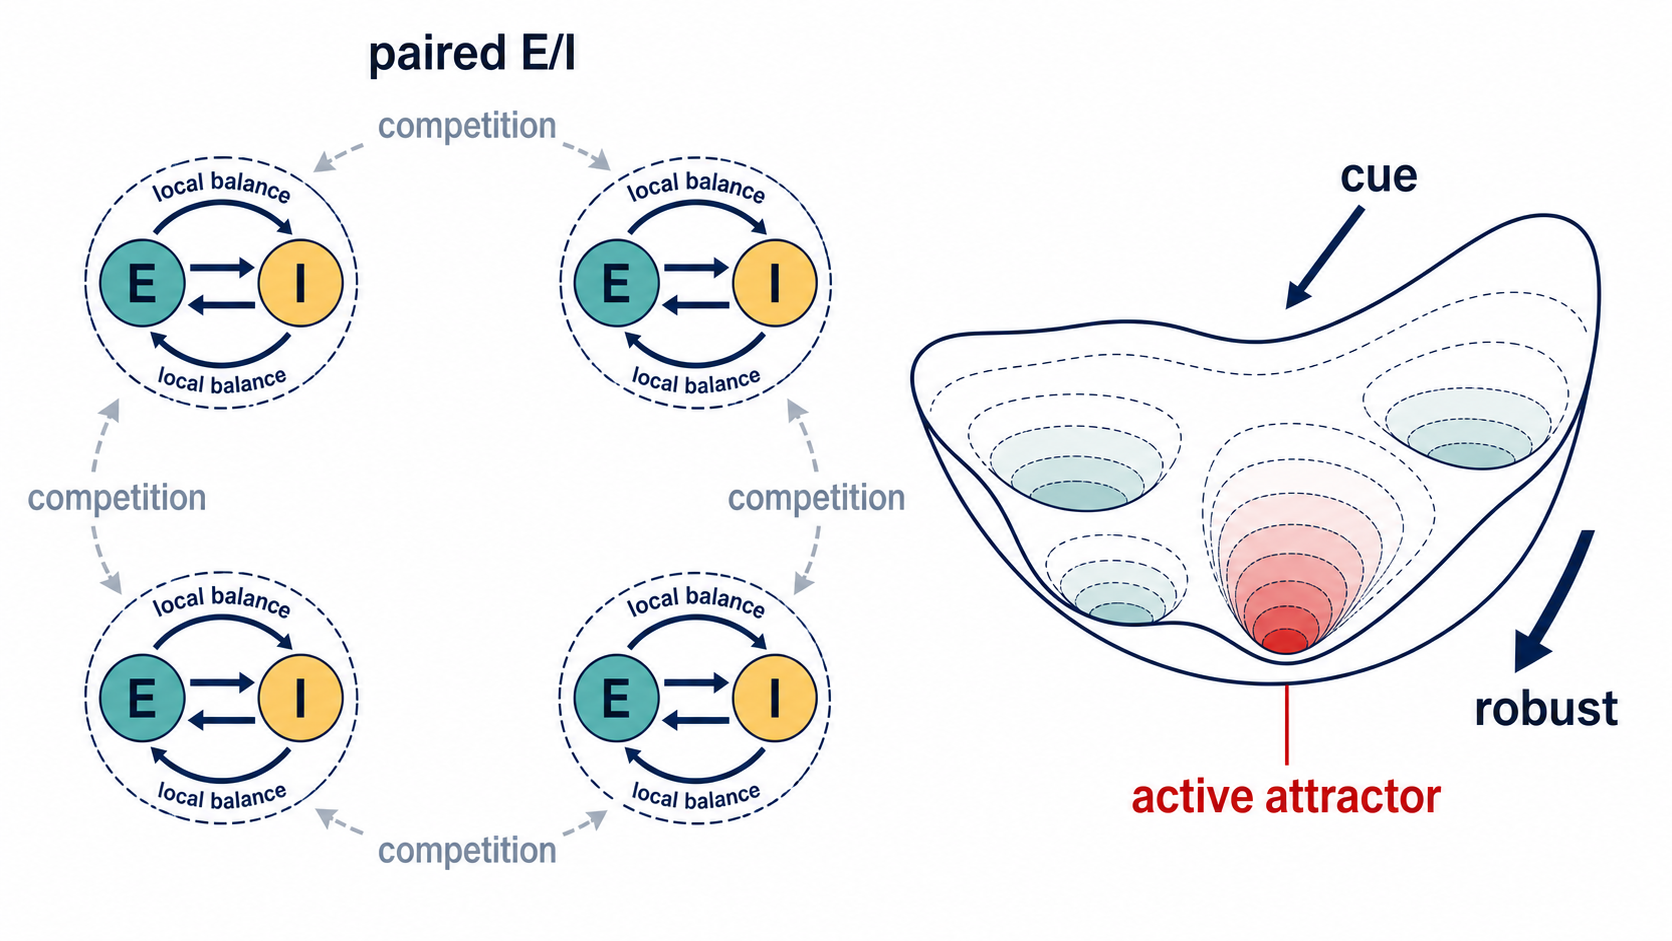
\includegraphics[width=0.95\textwidth]{figures/meso-rostami-paired-ei-clusters.png}
\caption{E/I clustered attractor models pair each excitatory cluster with a structured inhibitory partner. Local feedback can preserve balance inside an active state while competition separates candidate attractors. A cue tilts the landscape toward one basin without requiring the network to become globally regular.}
\label{fig:rostami-paired-ei-clusters}
\end{figure}

% ============================================================
\section{Why E/I Clustering Expands the Robust Parameter Regime}
\label{sec:ei-clustering-expands-robust-parameter-regime}
% ============================================================

In an E-only clustered network, cluster strength often has to do several jobs at once. It must support a high-rate state, create competition through shared inhibition, preserve irregular spiking, and avoid runaway activity. Those requirements can make metastability sensitive to a narrow range of excitatory recurrence.

E/I clustering adds a separate negative-feedback loop inside each active cluster. For one paired E/I cluster, a local linearization has the schematic Jacobian
%
\begin{equation}
  J_{\mathrm{pair}}
  =
  \begin{pmatrix}
    (-1+g_E W_+^{EE})/\tau_E &
    -g_E W_+^{EI}/\tau_E \\[0.6em]
    g_I W_+^{IE}/\tau_I &
    (-1-g_I W_+^{II})/\tau_I
  \end{pmatrix},
  \label{eq:rostami-pair-jacobian}
\end{equation}
%
where $g_E=\Phi_E'(u_E^*)$ and $g_I=\Phi_I'(u_I^*)$ are gains at the operating point. The term $g_E W_+^{EE}$ is positive feedback. The product $g_E W_+^{EI} g_I W_+^{IE}$ is a disynaptic E-to-I-to-E negative-feedback loop.

If inhibition is fast relative to excitation, one can approximate the local effective E recurrence by
%
\begin{equation}
  W_{\mathrm{eff}}^{EE}
  \approx
  W_+^{EE}
  -
  W_+^{EI}
  \frac{g_I}{1+g_I W_+^{II}}
  W_+^{IE}.
  \label{eq:rostami-effective-ee}
\end{equation}
%
The first term deepens the attractor. The second term subtracts local inhibitory feedback. Robustness can expand because $W_+^{EE}$ can be large enough to create an up-state while $W_+^{EI}$ and $W_+^{IE}$ limit gain, stabilize firing, and prevent explosive synchrony.

This is a mechanism-level explanation, not a theorem about all E/I clustered networks. E/I clustering helps only if the local inhibitory loop is strong and timed well enough to stabilize the attractor without suppressing it. The practical test is a phase diagram: measure the volume of parameter space in which rates are plausible, clusters switch on behavioral time scales, and single-neuron spiking remains irregular.

% ============================================================
\section{Explaining Task-Dependent Fano Factor Changes}
\label{sec:explaining-task-dependent-fano-factor-changes}
% ============================================================

Clustered attractor models explain task-dependent Fano factor changes through a mixture decomposition. Let $S(t)$ denote the latent cluster state or active-cluster pattern. Conditional on $S$, neuron $i$ has an approximate spike-count mean $\mu_i(S)$ and conditional variance $\sigma_i^2(S)$ in a fixed counting window. Across trials,
%
\begin{equation}
  \operatorname{Var}[N_i]
  =
  \mathbb{E}\!\left[\sigma_i^2(S)\right]
  +
  \operatorname{Var}\!\left[\mu_i(S)\right].
  \label{eq:fano-law-total-variance}
\end{equation}
%
The first term is within-state spiking variability. The second term is trial-to-trial variability caused by different trials occupying different cluster states. Dividing by $\mathbb{E}[N_i]$ gives the Fano factor:
%
\begin{equation}
  F_i
  =
  \frac{\mathbb{E}[\sigma_i^2(S)]}{\mathbb{E}[N_i]}
  +
  \frac{\operatorname{Var}[\mu_i(S)]}{\mathbb{E}[N_i]}.
  \label{eq:fano-decomposition-ch13}
\end{equation}
%
The two terms have different mechanisms. Local balanced spiking controls the first term. Attractor occupancy across trials controls the second term.

Prior target information reduces Fano factor if it reduces uncertainty about $S(t)$. When the prior specifies one target, trials are more likely to occupy a similar target-related basin before the go cue. Then $\operatorname{Var}[\mu_i(S)]$ decreases. When several targets remain possible, different trials can occupy different candidate basins, so the second term remains larger.

Stimulus- or cue-induced variability quenching is therefore not just a reduction in noise amplitude. It can be a reduction in latent-state diversity. The learner should measure both the Fano factor and the active-cluster occupancy distribution; a drop in Fano factor without a corresponding occupancy change would require a different explanation.

% ============================================================
\section{Why Spiking Irregularity Can Remain Roughly Constant}
\label{sec:why-spiking-irregularity-can-remain-constant}
% ============================================================

A reduction in across-trial Fano factor does not imply that neurons have become clock-like. The Fano factor in \eqref{eq:fano-decomposition-ch13} mixes slow latent-state variability and faster spiking variability. Measures such as $\operatorname{CV2}$ in \eqref{eq:cv2-ch13} focus more directly on the local irregularity of interspike intervals inside a trial.

Balanced E/I input can preserve irregular spiking across task epochs. Suppose the mean excitatory and inhibitory currents in state $S$ are both large:
%
\begin{equation}
  \mu_E(S)\approx \mu_I(S),
  \qquad
  |\mu_E(S)-\mu_I(S)| = O(1).
  \label{eq:balanced-current-scaling-ch13}
\end{equation}
%
The residual drive determines the firing rate, but the large fluctuating currents determine how irregular threshold crossings are. If task input changes the occupancy of attractor states while maintaining local E/I cancellation, the across-trial Fano factor can decrease while $\operatorname{CV2}$ remains roughly similar.

This distinction is important for judging the model. A model that explains Fano-factor quenching by simply reducing all noise might also predict more regular spike trains. The E/I clustered attractor hypothesis is sharper: task structure can reduce slow state variability while preserving irregular balanced spiking within each state.

% ============================================================
\section{What the Model Explains Mechanistically}
\label{sec:what-rostami-model-explains-mechanistically}
% ============================================================

The model gives a mechanistic chain from circuit architecture to behavior:
%
\begin{enumerate}[leftmargin=*]
  \item Paired E/I clusters create target-related attractor states.
  \item Finite-size fluctuations and recurrent competition produce metastable transitions among candidate states.
  \item Prior target information biases which basins are occupied during the delay.
  \item The go cue pushes the network toward the final target state.
  \item A readout threshold converts target-state separation into reaction time.
  \item Across-trial Fano factor changes because latent-state occupancy changes.
  \item Within-trial spiking irregularity can remain high because local balance is preserved.
\end{enumerate}

The model is therefore not only a fit to average firing rates. It proposes that variability itself is structured by the same attractor dynamics that support target selection. Slow trial-to-trial variability reflects which candidate state the network occupies; fast spike irregularity reflects the balanced spiking implementation of that state.

The strongest version of this claim requires simultaneous agreement across neural and behavioral observables. A model that matches reaction time but not Fano factors has not explained variability. A model that matches Fano factors but not target-dependent reaction time has not explained action selection.

% ============================================================
\section{What a Mesoscopic Version Should Preserve}
\label{sec:what-mesoscopic-version-should-preserve}
% ============================================================

A mesoscopic version should keep the variables and mechanisms needed for the explanation while removing unnecessary microscopic detail. The minimal state should include paired cluster activities
%
\begin{equation}
  \vec z(t)=
  (\vec r^{\,E}(t),\vec r^{\,I}(t)),
  \label{eq:mesoscopic-state-preserve-ch13}
\end{equation}
%
task inputs $h_{\alpha}(t)$, finite-size noise terms, and a decoder that maps cluster activity to reaction time. It should preserve the deterministic attractor skeleton, the finite-size fluctuation scale, and the mapping between target conditions and cluster drives.

The finite-size scaling should be explicit:
%
\begin{align}
  \mathrm{d}r_{\alpha}^{E}
  &=
  f_{\alpha}^{E}(\vec z;h)\,\mathrm{d}t
  +
  \frac{1}{\sqrt{n_{\alpha}^{E}}}
  \sum_{\mu}B_{\alpha\mu}^{E}(\vec z)\,\mathrm{d}W_{\mu}^{E},
  \label{eq:mesoscopic-e-noise-ch13}\\
  \mathrm{d}r_{\alpha}^{I}
  &=
  f_{\alpha}^{I}(\vec z;h)\,\mathrm{d}t
  +
  \frac{1}{\sqrt{n_{\alpha}^{I}}}
  \sum_{\mu}B_{\alpha\mu}^{I}(\vec z)\,\mathrm{d}W_{\mu}^{I}.
  \label{eq:mesoscopic-i-noise-ch13}
\end{align}
%
$n_{\alpha}^{E}$ and $n_{\alpha}^{I}$ control the noise strength of the E and I populations. If the model's switching is finite-size driven, changing these sizes while holding the deterministic drift fixed should change dwell times and reaction-time variability.

The mesoscopic model should match at least six observables:
%
\begin{enumerate}[leftmargin=*]
  \item mean rates of target-related clusters during baseline, delay, and response epochs;
  \item Fano factors and their task dependence;
  \item within-trial irregularity measures such as $\operatorname{CV2}$;
  \item cluster occupancy and lifetime distributions;
  \item reaction-time distributions across target-information conditions;
  \item scaling of switching with population size or added noise amplitude.
\end{enumerate}

It should not try to preserve every spike. The point of the reduction is to keep the variables that carry the explanation: cluster state, local E/I balance, finite-size noise, stimulus bias, and behaviorally relevant readout.

\begin{chaptersummary}

\begin{center}
\renewcommand{\arraystretch}{1.45}
\begin{tabularx}{\textwidth}{@{}l X X@{}}
  \toprule
  \textbf{Concept} & \textbf{Equation} & \textbf{Key Insight} \\
  \midrule
  Target uncertainty &
  $H(\mathcal{S})=\log|\mathcal{S}|$ &
  More possible targets means more candidate attractor states \\
  Task input &
  $h_{\alpha}=h_0+h_{\mathrm{prior}}\mathbf{1}_{\alpha\in\mathcal{S}}+h_{\mathrm{go}}\mathbf{1}_{\alpha=\alpha_*}$ &
  Prior and go cues bias different clusters \\
  Reaction time &
  $T_{\mathrm{RT}}=\inf\{t:y_{\alpha_*}-\max_{\beta\ne\alpha_*}y_{\beta}\ge\Theta\}$ &
  Selection is thresholded separation of the correct target state \\
  E/I cluster state &
  $\vec z=(\vec r^{\,E},\vec r^{\,I})$ &
  Each target-related state has excitatory and inhibitory population variables \\
  Local balance &
  $b_{\alpha}^{E}=h_{\alpha}^{E}+E_{\alpha}^{E}-I_{\alpha}^{E}$ &
  Large E and I currents can cancel to a controlled residual \\
  Fano decomposition &
  $\operatorname{Var}[N]=\mathbb{E}[\sigma^2(S)]+\operatorname{Var}[\mu(S)]$ &
  Slow latent-state variability and fast spiking variability are separable \\
  Mesoscopic preservation &
  $\mathrm{d}r=f\,\mathrm{d}t+n^{-1/2}B\,\mathrm{d}W$ &
  Finite-size scaling is part of the mechanism \\
  \bottomrule
\end{tabularx}
\end{center}

\end{chaptersummary}

\begin{conceptquestions}
  \item Why does target uncertainty naturally map onto a set of candidate attractor states rather than a single firing-rate level?

  \item In the reaction-time threshold \eqref{eq:reaction-time-threshold}, what does the competitor term $\max_{\beta\ne\alpha_*}y_{\beta}$ measure?

  \item Explain why a drop in Fano factor need not imply a drop in single-trial spiking irregularity.

  \item What is the difference between the residual drive $b_{\alpha}^{E}$ and the separate excitatory and inhibitory currents entering the same cluster?

  \item How does the decomposition \eqref{eq:fano-decomposition-ch13} connect latent attractor occupancy to trial-to-trial spike-count variability?

  \item Which microscopic details can be discarded in a mesoscopic Rostami-style model, and which cannot be discarded without losing the behavioral explanation?
\end{conceptquestions}
